\let\negmedspace\undefined
\let\negthickspace\undefined
\documentclass[journal]{IEEEtran}
\usepackage[a5paper, margin=10mm, onecolumn]{geometry}
%\usepackage{lmodern} % Ensure lmodern is loaded for pdflatex
\usepackage{tfrupee} % Include tfrupee package

\setlength{\headheight}{1cm} % Set the height of the header box
\setlength{\headsep}{0mm}     % Set the distance between the header box and the top of the text

\usepackage{gvv-book}
\usepackage{gvv}
\usepackage{cite}
\usepackage{amsmath,amssymb,amsfonts,amsthm}
\usepackage{algorithmic}
\usepackage{graphicx}
\usepackage{textcomp}
\usepackage{xcolor}
\usepackage{txfonts}
\usepackage{listings}
\usepackage{enumitem}
\usepackage{mathtools}
\usepackage{gensymb}
\usepackage{comment}
\usepackage[breaklinks=true]{hyperref}
\usepackage{tkz-euclide} 
\usepackage{listings}
% \usepackage{gvv}                                        
\def\inputGnumericTable{}                                 
\usepackage[latin1]{inputenc}                                
\usepackage{color}                                            
\usepackage{array}                                            
\usepackage{longtable}                                       
\usepackage{calc}                                             
\usepackage{multirow}                                         
\usepackage{hhline}                                           
\usepackage{ifthen}                                           
\usepackage{lscape}
\begin{document}

\bibliographystyle{IEEEtran}
\vspace{3cm}

\title{NCERT 9.1.4}
\author{EE24BTECH11036 - Krishna Patil}

% \maketitle
% \newpage
% \bigskip
{\let\newpage\relax\maketitle}

\renewcommand{\thefigure}{\theenumi}
\renewcommand{\thetable}{\theenumi}
\setlength{\intextsep}{10pt} % Space between text and floats


\textbf{Question:} Solve the ODE \((\frac{d^2y}{dx^2})^2 + \cos\left(\frac{dy}{dx}\right) = 0.\)

\solution
The given equation is:
\[
\left(\frac{d^2y}{dx^2}\right)^2 + \cos\left(\frac{dy}{dx}\right) = 0.
\]

\begin{enumerate}
    \item \textbf{Reformulate the equation:}
    Define \(v = \frac{dy}{dx}\) and \(u = \frac{d^2y}{dx^2}\). The equation becomes:
    \[
    u^2 + \cos(v) = 0.
    \]
    Solving for \(u\), we get:
    \[
    u = \pm \sqrt{-\cos(v)}, \quad \text{valid only for } \cos(v) < 0.
    \]

    Thus, the system of equations is:
    \[
    \frac{dy}{dx} = v, \quad \frac{dv}{dx} = u = \pm \sqrt{-\cos(v)}.
    \]

    \item \textbf{Update equations for \(y\):}
    Using the RK4 method, the update for \(y\) is:
    \begin{align*}
        k_{y,1} &= h \cdot v, \\
        k_{y,2} &= h \cdot \left(v + \frac{k_{v,1}}{2}\right), \\
        k_{y,3} &= h \cdot \left(v + \frac{k_{v,2}}{2}\right), \\
        k_{y,4} &= h \cdot \left(v + k_{v,3}\right), \\
        y_{n+1} &= y_n + \frac{1}{6}\left(k_{y,1} + 2k_{y,2} + 2k_{y,3} + k_{y,4}\right).
    \end{align*}

    \item \textbf{Update equations for \(v\):}
    Using the RK4 method for \(v\), we have:
    \begin{align*}
        k_{v,1} &= h \cdot \sqrt{-\cos(v)}, \\
        k_{v,2} &= h \cdot \sqrt{-\cos\left(v + \frac{k_{v,1}}{2}\right)}, \\
        k_{v,3} &= h \cdot \sqrt{-\cos\left(v + \frac{k_{v,2}}{2}\right)}, \\
        k_{v,4} &= h \cdot \sqrt{-\cos\left(v + k_{v,3}\right)}, \\
        v_{n+1} &= v_n + \frac{1}{6}\left(k_{v,1} + 2k_{v,2} + 2k_{v,3} + k_{v,4}\right).
    \end{align*}

    \item \textbf{Numerical Implementation:}
    The numerical solution proceeds by alternating updates for \(y\) and \(v\), using the equations above. Choose initial values \(y(0) = y_0\) and \(v(0) = v_0\), and iterate using a step size \(h\).
\end{enumerate}

\textbf{Summary of the Two-Step RK4 Process:}
- Update \(y\) using \(k_{y,1}, k_{y,2}, k_{y,3}, k_{y,4}\).
- Update \(v\) using \(k_{v,1}, k_{v,2}, k_{v,3}, k_{v,4}\).

\textbf{Note:} Ensure that the step size \(h\) is small enough to maintain accuracy and stability.

Below is the plot \figref{fig:example}.

\begin{figure}[h]
    \centering
    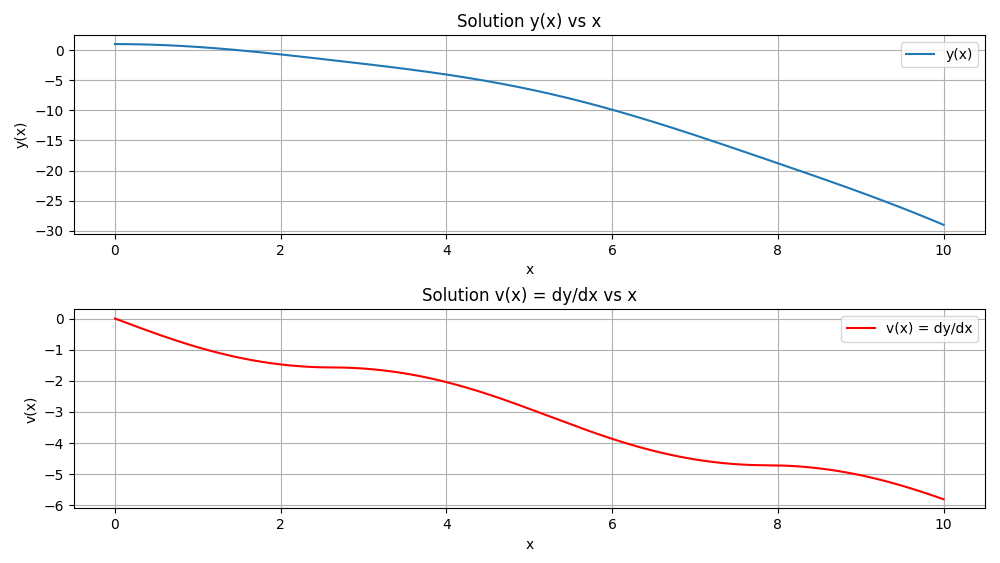
\includegraphics[width=\columnwidth]{fig/Figure_1.png}
    \caption{Verification}
    \label{fig:example}
\end{figure}

\end{document}

\end{document}

